\documentclass[11pt]{beamer}

% ---------------------------------------------------------------------
% Preamble
% ---------------------------------------------------------------------

% ---------------------------------------------------------------------
% Packages
% ---------------------------------------------------------------------

\usepackage[utf8]{inputenc}
\usepackage{amsmath}
\usepackage{amssymb}
\usepackage[ngerman]{babel}
\usepackage{beamerprosper}
\usepackage{color}
\usepackage{epsfig}
\usepackage{graphicx}
\usepackage{epsfig}
\usepackage{latexsym}
\usepackage{listings}
\usepackage{times}
\usepackage{url}
\usepackage{xspace}
\usepackage{pgfpages}

% ---------------------------------------------------------------------
% Spacings
% ---------------------------------------------------------------------

\setlength{\parskip}{0.5ex}

% ---------------------------------------------------------------------
% Settings
% ---------------------------------------------------------------------

\lstset{ %
  backgroundcolor=\color{white},   % choose the background color; you must add \usepackage{color} or \usepackage{xcolor}
  basicstyle=\footnotesize\ttfamily, % the size of the fonts that are used for the code
  breakatwhitespace=false,         % sets if automatic breaks should only happen at whitespace
  breaklines=true,                 % sets automatic line breaking
  captionpos=b,                    % sets the caption-position to bottom
  commentstyle=\color{green},  	   % comment style
  deletekeywords={...},            % if you want to delete keywords from the given language
  escapeinside={\%*}{*)},          % if you want to add LaTeX within your code
  extendedchars=true,              % lets you use non-ASCII characters; for 8-bits encodings only, does not work with UTF-8
  frame=single,                    % adds a frame around the code
  keepspaces=true,                 % keeps spaces in text, useful for keeping indentation of code (possibly needs columns=flexible)
  keywordstyle=\color{blue},       % keyword style
  language=Java,                   % the language of the code
  morekeywords={*,...},            % if you want to add more keywords to the set
  numbers=left,                    % where to put the line-numbers; possible values are (none, left, right)
  numbersep=5pt,                   % how far the line-numbers are from the code
  numberstyle=\tiny\color{green},  % the style that is used for the line-numbers
  rulecolor=\color{black},         % if not set, the frame-color may be changed on line-breaks within not-black text (e.g. comments (green here))
  showspaces=false,                % show spaces everywhere adding particular underscores; it overrides 'showstringspaces'
  showstringspaces=false,          % underline spaces within strings only
  showtabs=true,                   % show tabs within strings adding particular underscores
  stepnumber=1,                    % the step between two line-numbers. If it's 1, each line will be numbered
  stringstyle=\color{blue},        % string literal style
  tabsize=2,                       % sets default tabsize to 2 spaces
  title=\lstname                   % show the filename of files included with \lstinputlisting; also try caption instead of title
}

% ---------------------------------------------------------------------
% Paths
% ---------------------------------------------------------------------

\graphicspath{{./images/}}

% ---------------------------------------------------------------------
% Theme
% ---------------------------------------------------------------------

\mode<all>
\usetheme{CambridgeUS}
\mode<presentation>
{
  \useinnertheme{rectangles}
  %\useoutertheme{}
  \setbeamercovered{transparent}
  \setbeamertemplate{navigation symbols}{}
}

% \definecolor{darkred}{rgb}{0.625,0.125,0.25}
\definecolor{darkred}{rgb}{0,0.4196,0.5803}
% \definecolor{bauhausblue}{rgb}{0,0.107,0.148}

\setbeamercolor{block body}{bg=gray!20}
\setbeamercolor{block title}{bg=darkred,fg=white}
\setbeamercolor{footlinecolorl}{fg=black,bg=lightgray}
\setbeamercolor{footlinecolor}{fg=black,bg=gray}
\setbeamercolor{footlinecolord}{fg=black,bg=darkgray}

\setbeameroption{show notes}
\setbeameroption{show notes on second screen=right}

% Auskommentieren, für Section 1,2,3, ...
\setbeamertemplate{section page}
{
    \begin{centering}
    \begin{beamercolorbox}[sep=12pt,center]{part title}
    \usebeamerfont{section title}\insertsection\par
    \end{beamercolorbox}
    \end{centering}
}

\setbeamertemplate{footline}{%
	\hbox{%
	\begin{beamercolorbox}[wd=.40\paperwidth,ht=4.25ex,left,leftskip=3ex]{author in head/foot}%
	    \vbox to4.25ex{\vfil\hbox{\usebeamerfont{author in head/foot} \insertshortauthor}\vfil}%
	\end{beamercolorbox}%
	\begin{beamercolorbox}[wd=.30\paperwidth,ht=4.25ex,center]{title in head/foot}%
	    \vbox to4.25ex{\vfil\hbox{\usebeamerfont{date in head/foot}\insertshorttitle{}}\vfil}%
	\end{beamercolorbox}%
  % \begin{frame number}{}
  % \end{frame number}%
	\begin{beamercolorbox}[wd=.30\paperwidth,ht=4.25ex,right,rightskip=3ex]{date in head/foot}%
	    % \vbox to4.25ex{\vfil\hbox{\insertshortdate{}}\vfil}%
      % \vbox to4.25ex{\vfill\hbox{frame number}}
      \vbox to4.25ex{\vfill\hbox{\insertframenumber{} / \inserttotalframenumber }\vfill}
	\end{beamercolorbox}}%
}
%\setbeamertemplate{footline}{
%  \quad \tiny \insertshortauthor \hfill \insertshorttitle \qquad \hfill \insertshortdate\ \qquad\qquad
%}
\setbeamertemplate{theorems}[numbered]
% ---------------------------------------------------------------------
% Commands
% ---------------------------------------------------------------------

\newcommand{\eg}{\textit{e.g.,}\xspace}
\newcommand{\shortsep}{||}
\newcommand{\sep}{\ \shortsep \ }
\def\getpdfpages#1#2{\begingroup
  \setbeamercolor{background canvas}{bg=}
  \includepdf[pages={#1},%
  pagecommand={\global\setcounter{framenumber}{\value{page}}%
    \expandafter\def\expandafter\insertshorttitle\expandafter{%
      \insertshorttitle\hfill\insertframenumber\,/\,\inserttotalframenumber}}%
  ]{#2}
  \endgroup}

% ---------------------------------------------------------------------
% Title
% ---------------------------------------------------------------------

\title[Bauhausboards]{Bauhausboards\\Interactive Door Signs for the Office}
\subtitle{Bachelorverteidigung}
\author[André Karge]{André Karge}
\institute[Bauhaus-Universität Weimar]{
\includegraphics[width=0.5\textwidth]{buw-logo}}
\date[29.02.2016]{29.02.2016}

\raggedright
\AtBeginSection{\frame{\sectionpage}}

% ---------------------------------------------------------------------

\begin{document}

% ---------------------------------------------------------------------
% Content
% ---------------------------------------------------------------------

\maketitle

\begin{frame}{Agenda}
\tableofcontents
\end{frame}
% ---------------------------------------------------------------------
\section{Grundlagen}
% - Einführung in Interaktive Türschilder
% - Netboards als Vorlageprojekt
%   * ein wenig Netboards erklären
% - Entscheidungspunkt: Eigenes System "Bauhausboards" entwickeln
\begin{frame}{Arbeit}
  % Ziel der Arbeit:
  % \begin{itemize}
  %   \item Erstellung
  % \end{itemize}
  % \begin{center}
    System zur \textbf{Kommunikation} und \textbf{Präsentation} von Daten im Bürobereich
    \pause
    \begin{itemize}
      \item Tablets neben Büroeingängen
      \item Ablösung herkömmlicher Türschilder
    \end{itemize}
  % \end{center}
  \note<1-2>{
    \begin{itemize}
      \item befasste mich in Arbeit:
      \item erstellung System zur Kommunikation + Präsentation von Daten im Bürobereich
      \item System sollte auf neben Büros angebrachten Tablets basieren
      \item $\rightarrow$ soll herkömmliche Türschilder als Informationsquelle ablösen
    \end{itemize}
  }
\end{frame}

\begin{frame}{Türschilder}
  Nutzung von Türschildern in Forschungseinrichtungen
  \note<1>{
    \begin{itemize}
      \item in Forschungseinrichtungen: Türschilder als Info-Schnittstelle zw. Mitarbeiter im Büro - Gästen/Kollegen genutzt
    \end{itemize}
    Das sind:\\
    \begin{itemize}
      \item Whiteboards
      \item Tafeln
      \item Post-It Zettel
      \item Bitte-Nicht-Stören-Schilder
    \end{itemize}
  }
  \pause
  \begin{itemize}
    \item Darbietung aller Art von Informationen
    \item Kommunikation zwischen Mitarbeitern und Gästen
    \note<2>{
      Dienen zur:
      \begin{itemize}
        \item Darbietung persönlicher Daten (sind Informationen aller Art)
        \begin{itemize}
          \item Handskizzen
          \item Texte
          \item Ausdrucke
          \item Statusmeldungen (bspw.: bin gleich wieder da / die ganze Woche auf Forschungsreise)
        \end{itemize}
      \end{itemize}
    }
    % \pause
    \note<2>{
      \begin{itemize}
        \item Informationen dienen: Informationsangebot oder Kommunikation
        \begin{itemize}
          \item an was arbeiten die Kollegen in den Büros / gibt es Veranstaltungen
          \item das heißt: Forschungsarbeit / aktuelles Paper / Projekt / Termine
          \item Oder: Nutzung für Auflockernden Inhalt (Comics / Skizzen)
        \end{itemize}
      \end{itemize}
    }
  \end{itemize}
    % - Darbietung von persönlichen Daten (Informationen aller Art - Handskizzen, Texte, Ausdrucke, Statusmeldungen(bin gleich wieder da))
    % - Kommunikation zwischen Mitarbeitern / Gästen
\end{frame}

\begin{frame}
  % \todo{hier ein Bild von einem Whiteboard in der B11}
  \begin{center}
    Aktuelle Situation?\\~\\
    \pause
    \visible<2>{
      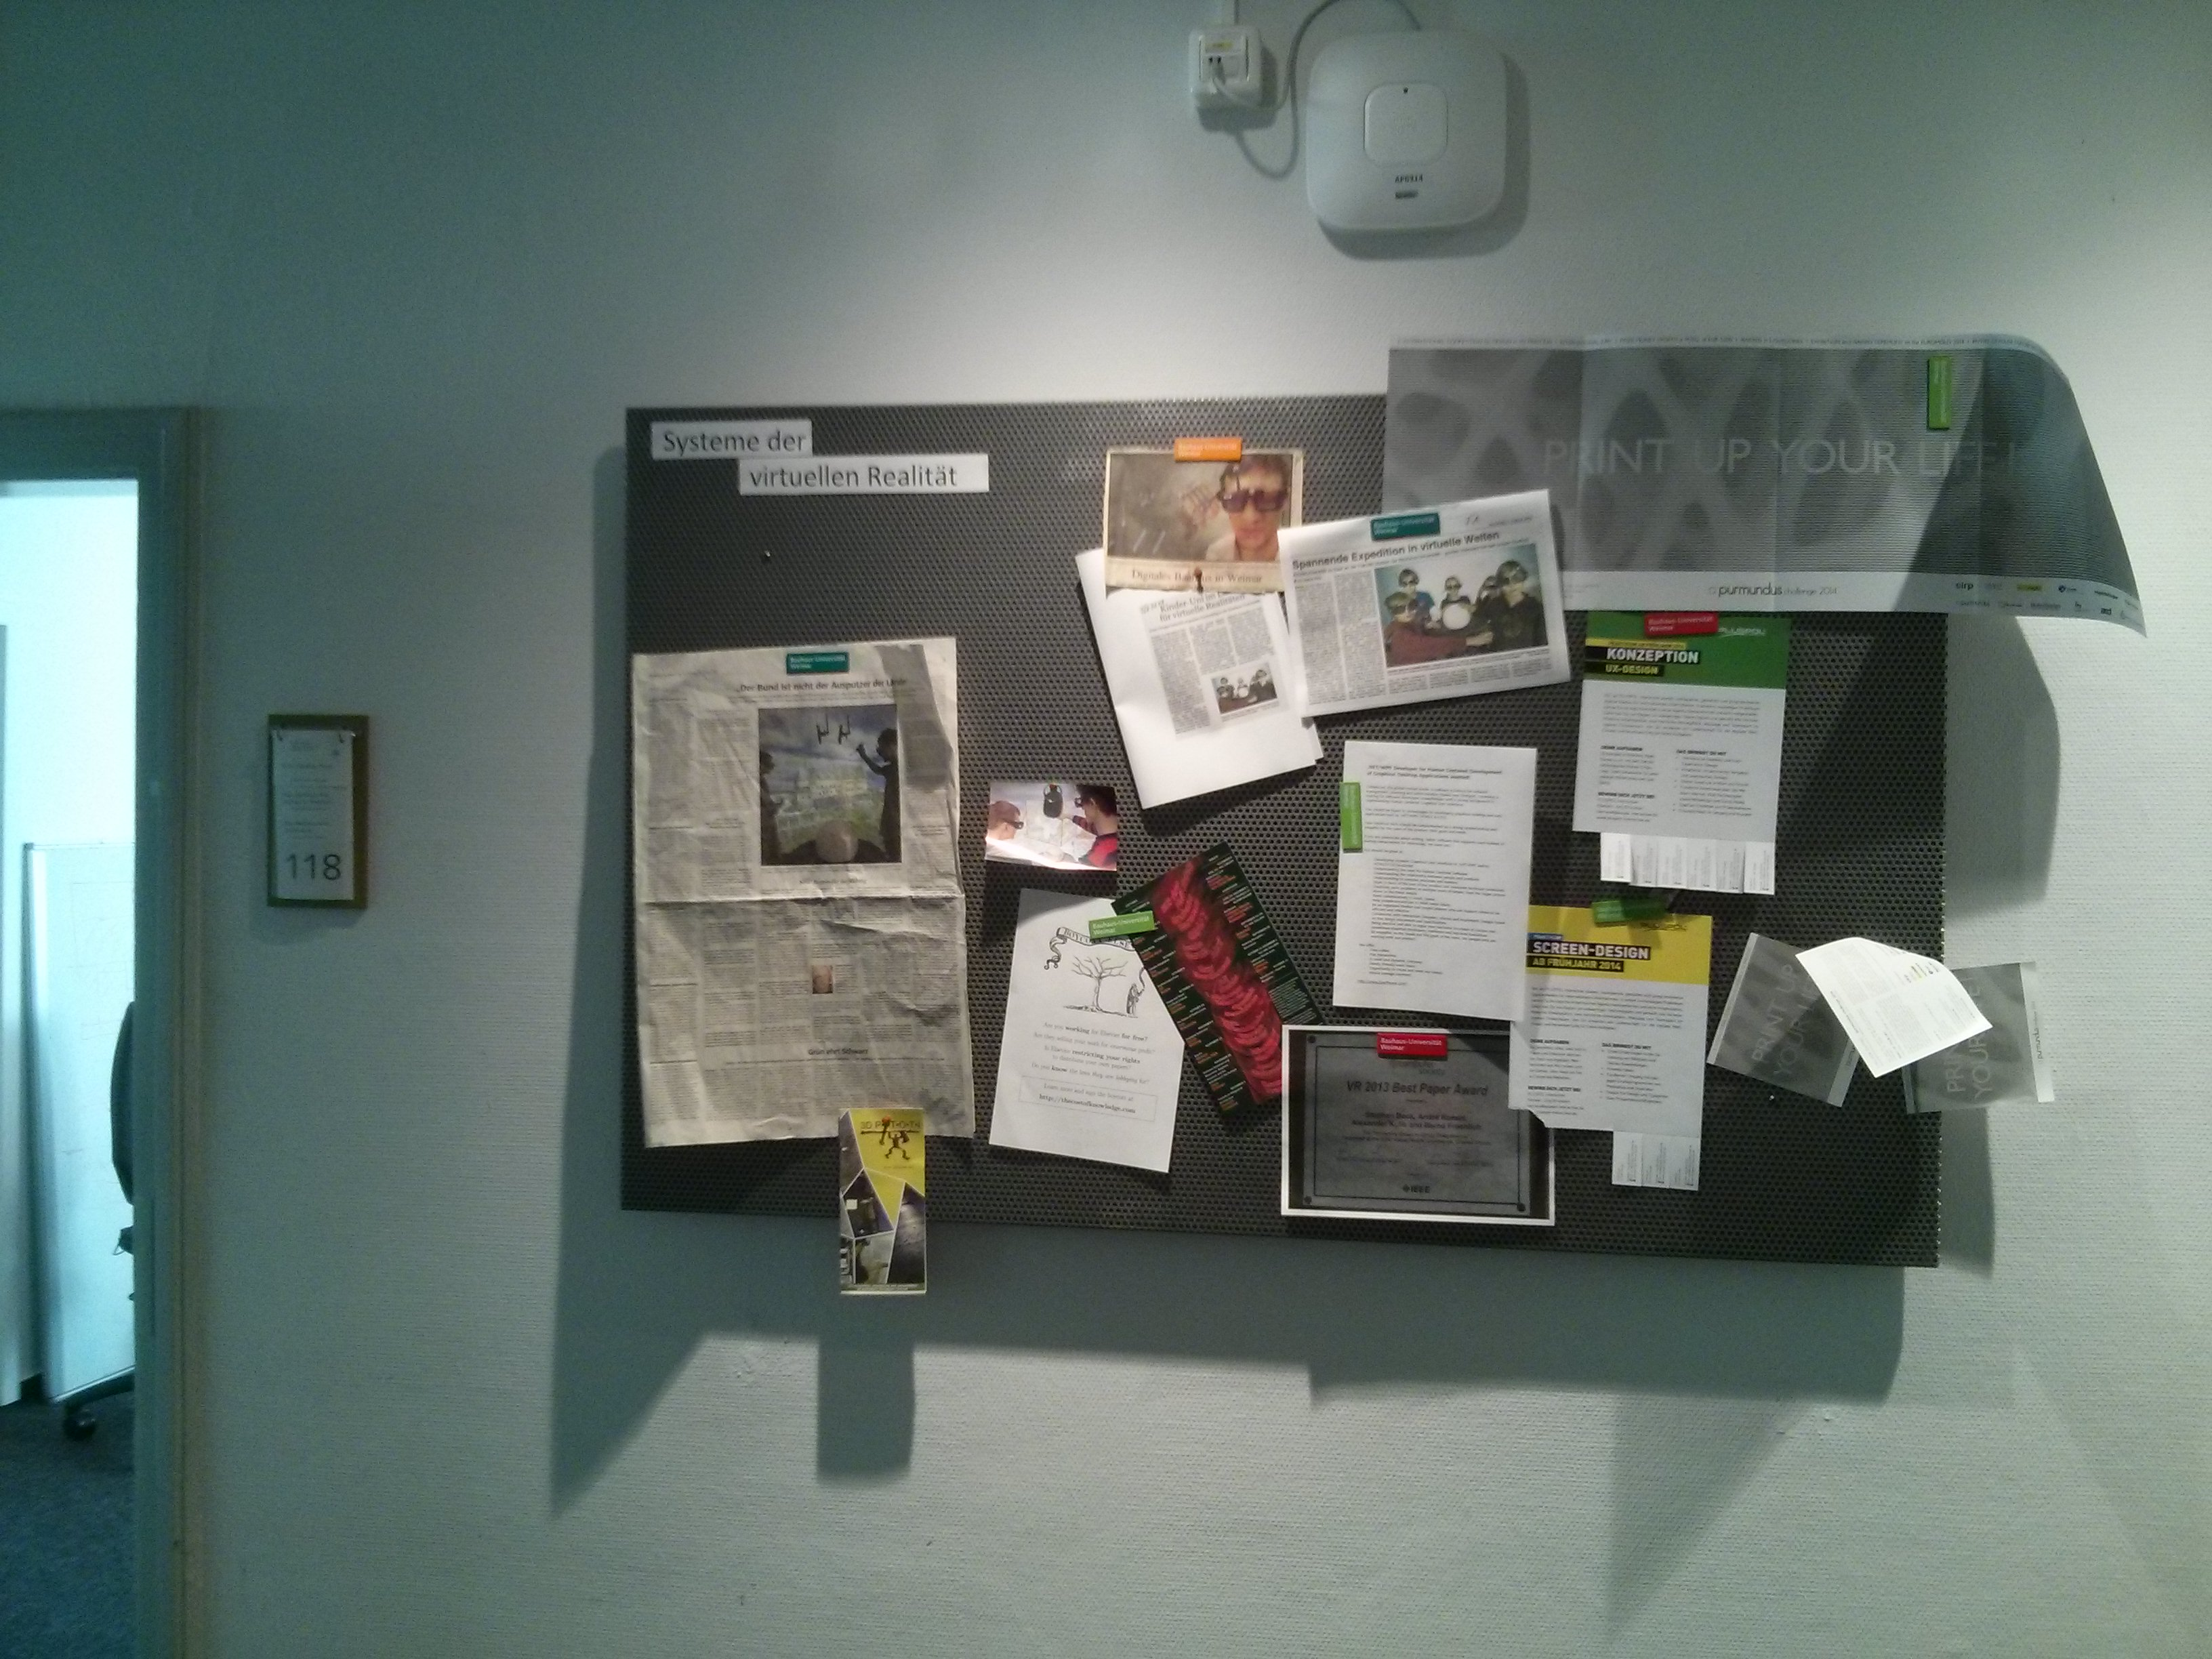
\includegraphics[width=0.6\textwidth]{pinnwand}\\
      \quelle{Quelle: HCI-Pinnwand Bauhausstraße 11}
    }
  \end{center}
  \note<1-2>{
    Aber: Wie sieht das aktuell aus? -click-\\
    diese Form der Informationsdarbietung: gewisse Nachteile -click-
  }
\end{frame}

\begin{frame}{Nachteile}
  \begin{columns}
    \begin{column}{0.49\textwidth}
      Nachteile von analogen Türschildern:
      % \pause
      \visible<2-3>{
        \begin{itemize}
          \item Man muss persönlich vor Ort sein
          % \pause
          \visible<3>{
            \item Ungewünschtes Entfernen / Hinzufügen / Ändern von Informationen durch Dritte
          }
        \end{itemize}
      }
    \end{column}
    \visible<1-3>{
      \begin{column}{0.49\textwidth}
        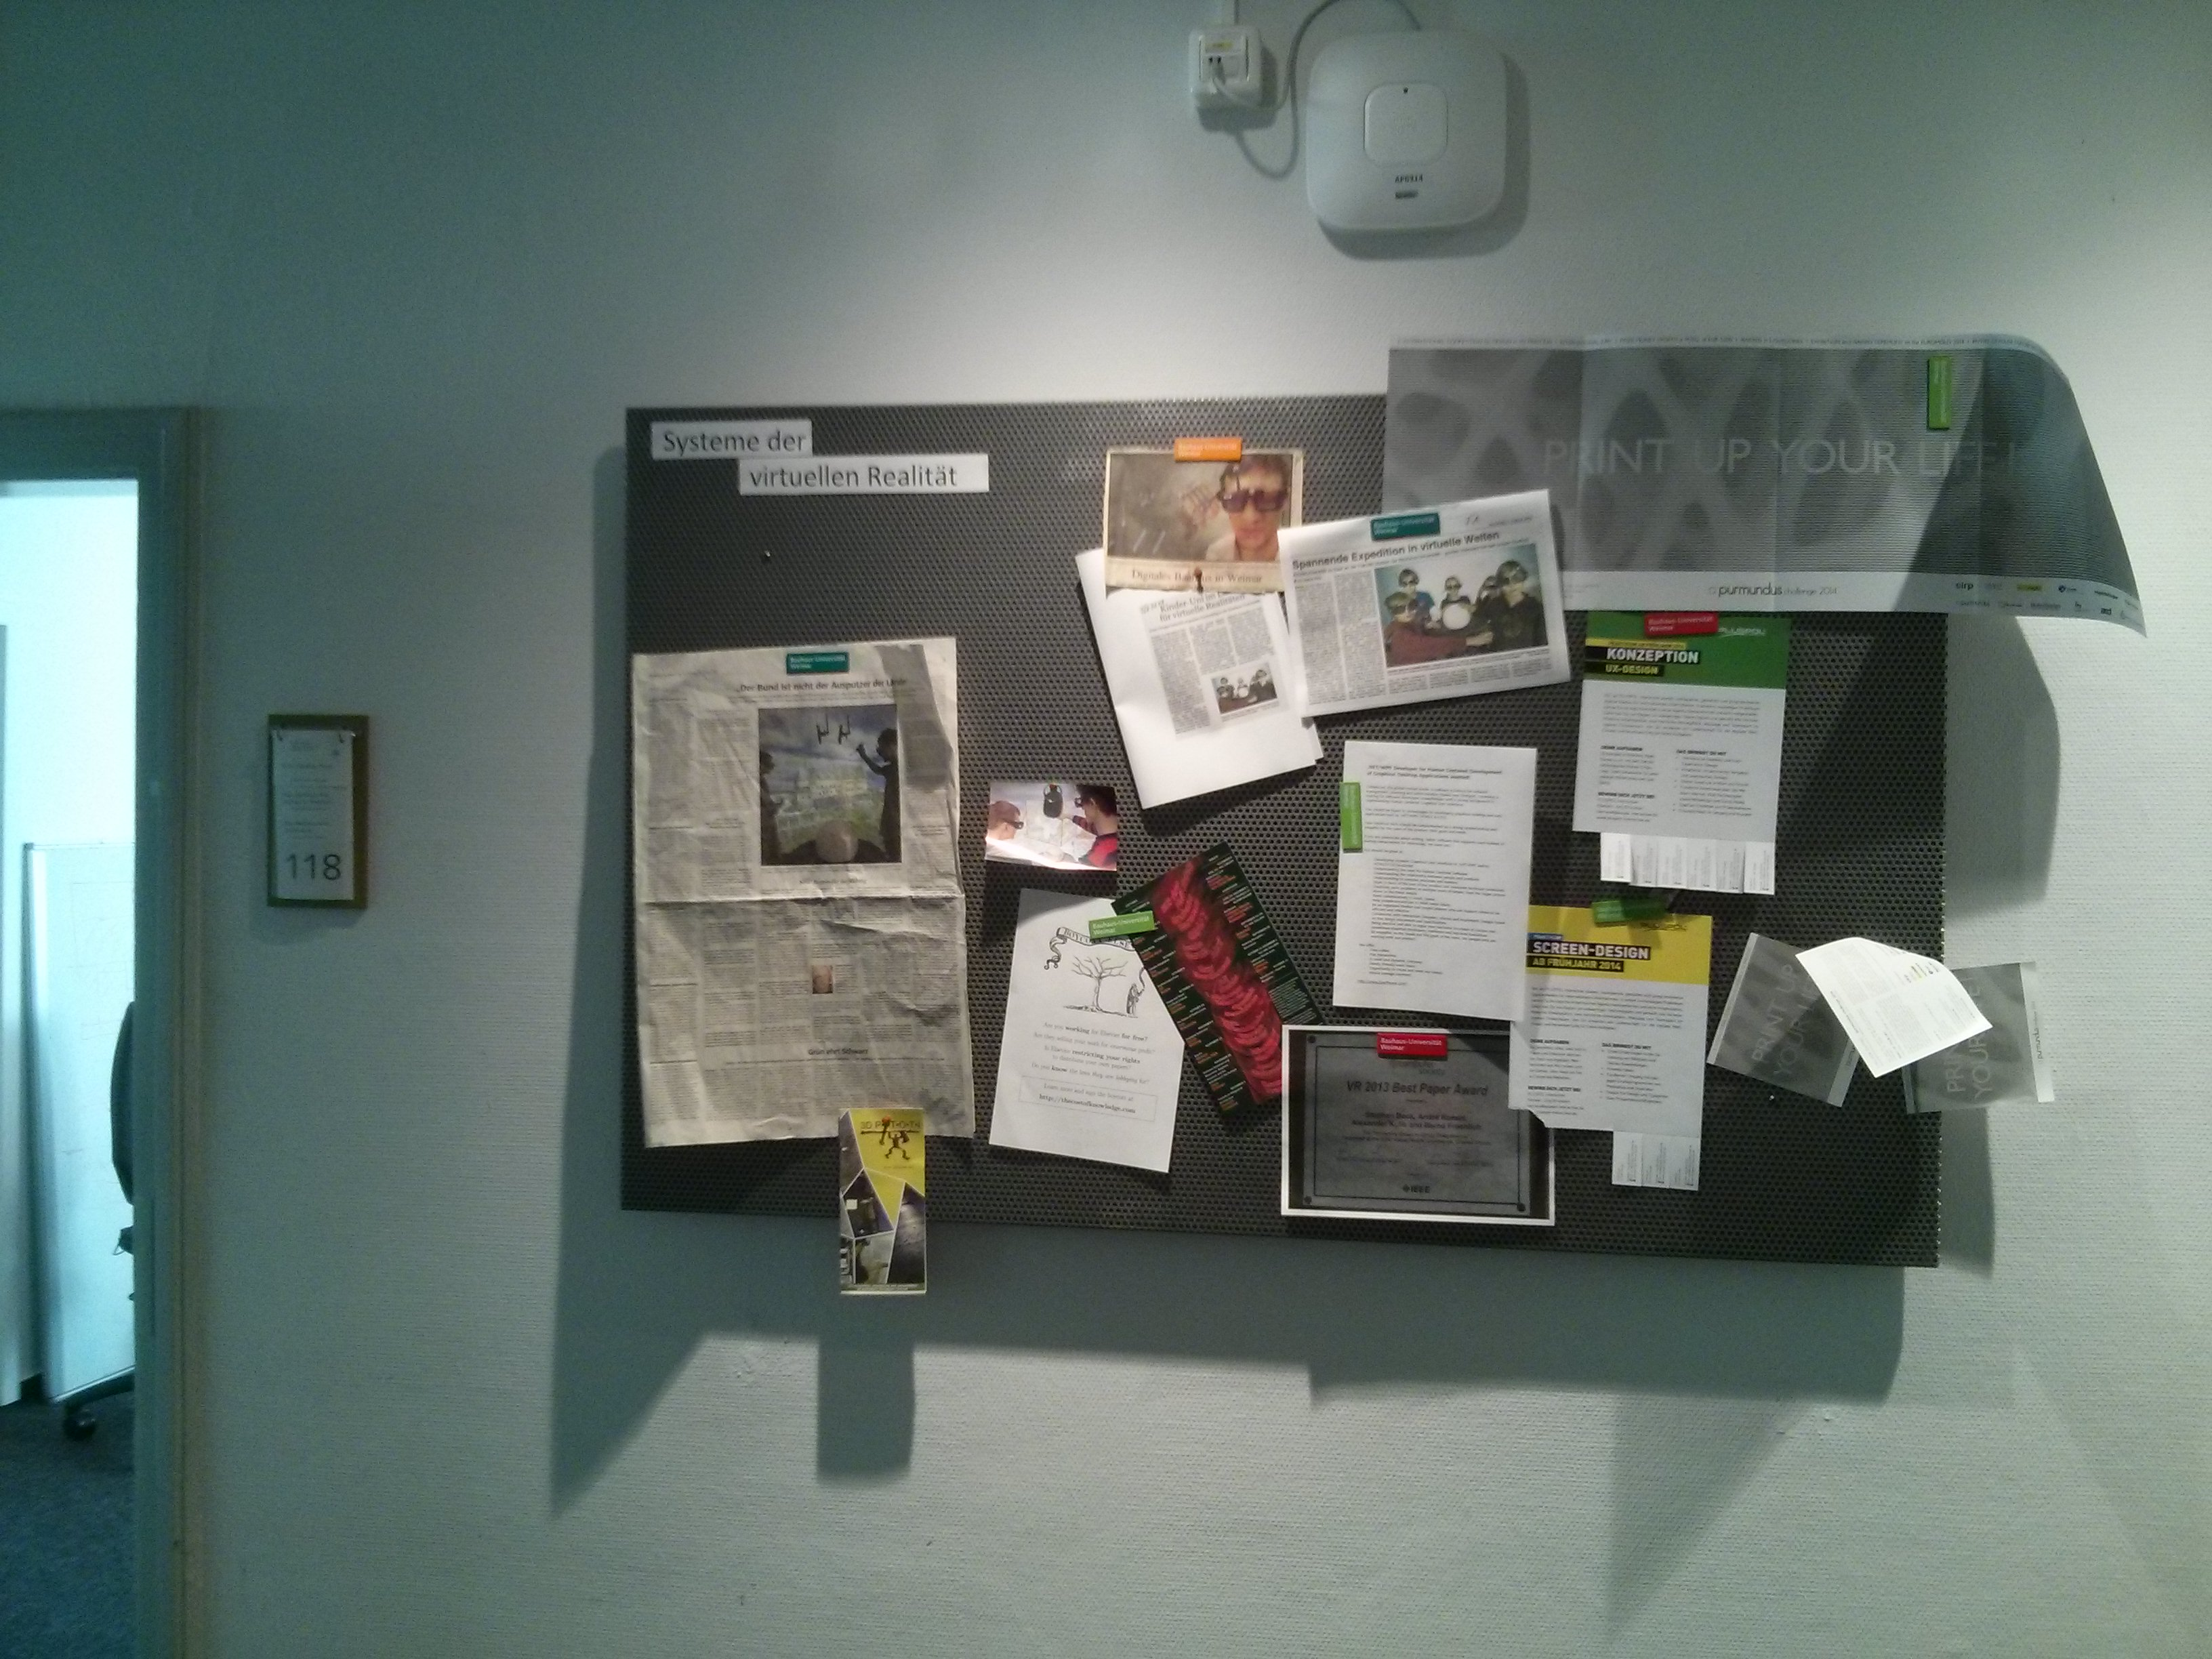
\includegraphics[width=0.9\textwidth]{pinnwand}
      \end{column}
    }
  \end{columns}
  % Nachteile von analogen Türschildern:
  % \pause
  % \begin{itemize}
  %   \item Man muss persönlich vor Ort sein
  %   \pause
  %   \item Ungewünschtes Entfernen / Hinzufügen / Ändern von Information durch Dritte
  % \end{itemize}
  \note<1>{
    zum einen: persönlich vor Ort sein -click-
  }
  \note<2>{
    \begin{itemize}
      \item Änderung Inhaltes nur: wenn selbst im Büro
      \item Oder: Beauftragung eines Kollegen mit Änderung
      \item selbes auch bei hinterlassenen Nachrichten
    \end{itemize}
  }
  \note<3>{
    \begin{itemize}
      \item jeder Vorbeigehende kann nach Belieben Texte/Bilder ändern/hinzufügen/entfernen
      \item $\rightarrow$ Möglichkeit von Vandalismus sehr hoch
      \item (Mensa: aus Rinderhacksteak $\rightarrow$ Kinderhacksteak)
    \end{itemize}
  }
    % - Content kann nur geändert werden, wenn man persönlich vor Ort ist
    % - Hinterlassene Nachrichten können nur gelesen werden, wenn man selbst vor Ort ist
    % - Zudem können Gäste den bestimmte Sachen abwischen / neue hinzufügen (Vandalismus)
\end{frame}
\begin{frame}{Lösung}
  \note<1>{
    Eine Lösung ist das Anbringen von interaktiven digitalen Türschildern
  }
  Anbringung von digitalen Türschildern
    \pause
    \begin{itemize}
      \item Änderung von präsentierten Inhalten aus der Ferne
      \item Erhalt von Gästemitteilungen ohne vor Ort zu sein
      \item Einschränkung von Vandalismus
    \end{itemize}
  \note<2>{
    \begin{itemize}
      \item Vorteil: man muss nicht mehr selbst vor Ort sein um Inhalt zu ändern / Nachrichten zu erhalten
      \item Durch Eingrenzung der Interaktionsmöglichkeiten: Einschränkung von Vandalismus (Nutzungsrechte)
    \end{itemize}
  }
    % - Interaktive Türschilder
    % - Digitaler Ersatz für Whiteboards/Tafeln neben Büros
    % - Nutzer müssen nicht mehr persönlich vor Ort sein, um Content zu ändern / Nachrichten zu empfangen
    % - Vandalismus wird eingeschränkt
\end{frame}

\begin{frame}[t]{Vorarbeit}
  \note<1-3>{
    Dazu: einige Projekte mit ähnlichem Ansatz:
    \begin{itemize}
      \item Hermes Universität Lancaster (etwas älteres Projekt) (2003)
      \item NetBoards Universität Cambridge (aktuelleres Projekt) (2014)
    \end{itemize}
    NetBoards in Vorstudie ausprobiert. -click-
  }
  \pause
  \begin{columns}[t]
    \begin{column}{0.49\textwidth}
      \begin{center}
        \visible<2-3>{
          Hermes (2003)\\
          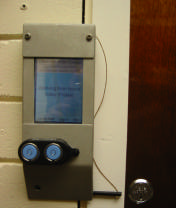
\includegraphics[width=0.7\textwidth]{hermes_display}\\
          \quelle{Quelle: Keith Cheverest et. al. - Ambient Intelligence 2003}
        }
      \end{center}
    \end{column}
    \pause
    \visible<3>{
      \begin{column}{0.49\textwidth}
        \begin{center}
          NetBoards (2014)\\
          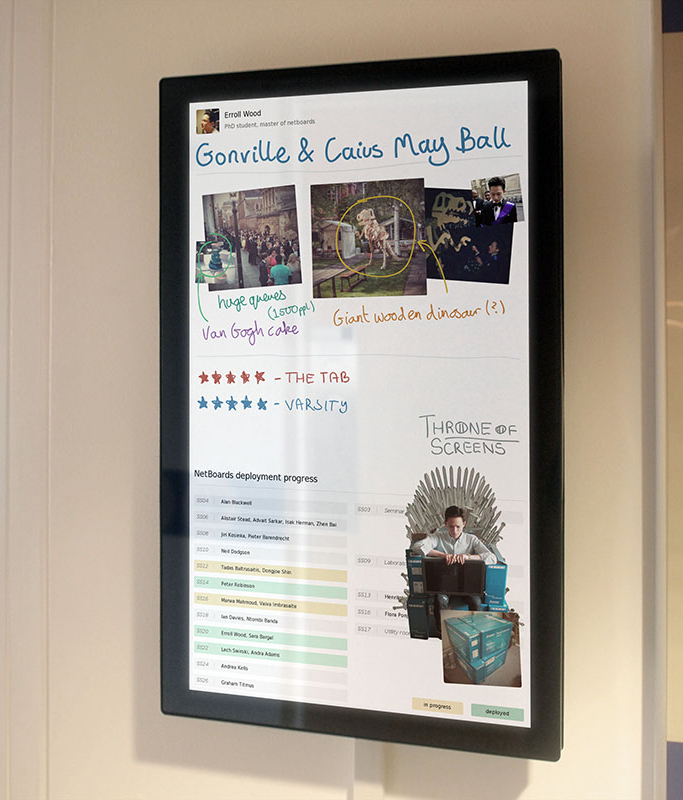
\includegraphics[width=0.705\textwidth]{netboards}\\
          \quelle{Quelle: Errol Wood et. al. - ACM ITS 2014}\\
        \end{center}
      \end{column}
    }
  \end{columns}
  % \pause
  % NetBoards in kleiner Studie aufgesetzt\\
  % Als Ergebnis: eigenes Projekt

  %   - Hermes (2003)
  %   - Netboards (2014)
  % - Ergebnis aus Vorstudie mit NetBoards: eigenes Projekt
\end{frame}

\begin{frame}{Vorstudie}
  \begin{columns}
    \begin{column}{0.59\textwidth}
      Ziel:
      \begin{itemize}
        \item Anforderungsanalyse
      \end{itemize}
      \visible<2-3>{
        Ergebnis:
        \begin{itemize}
          \item Tablets erzeugten viel Aufmerksamkeit
          \item Zu offene Interaktivität
          \item Häufig unerwünschter Inhalt (Vandalismus)
        \end{itemize}
        }
      \visible<3>{
        $\rightarrow$ Aufsetzen eines eigenen Projektes
      }
    \end{column}
    \begin{column}{0.39\textwidth}
      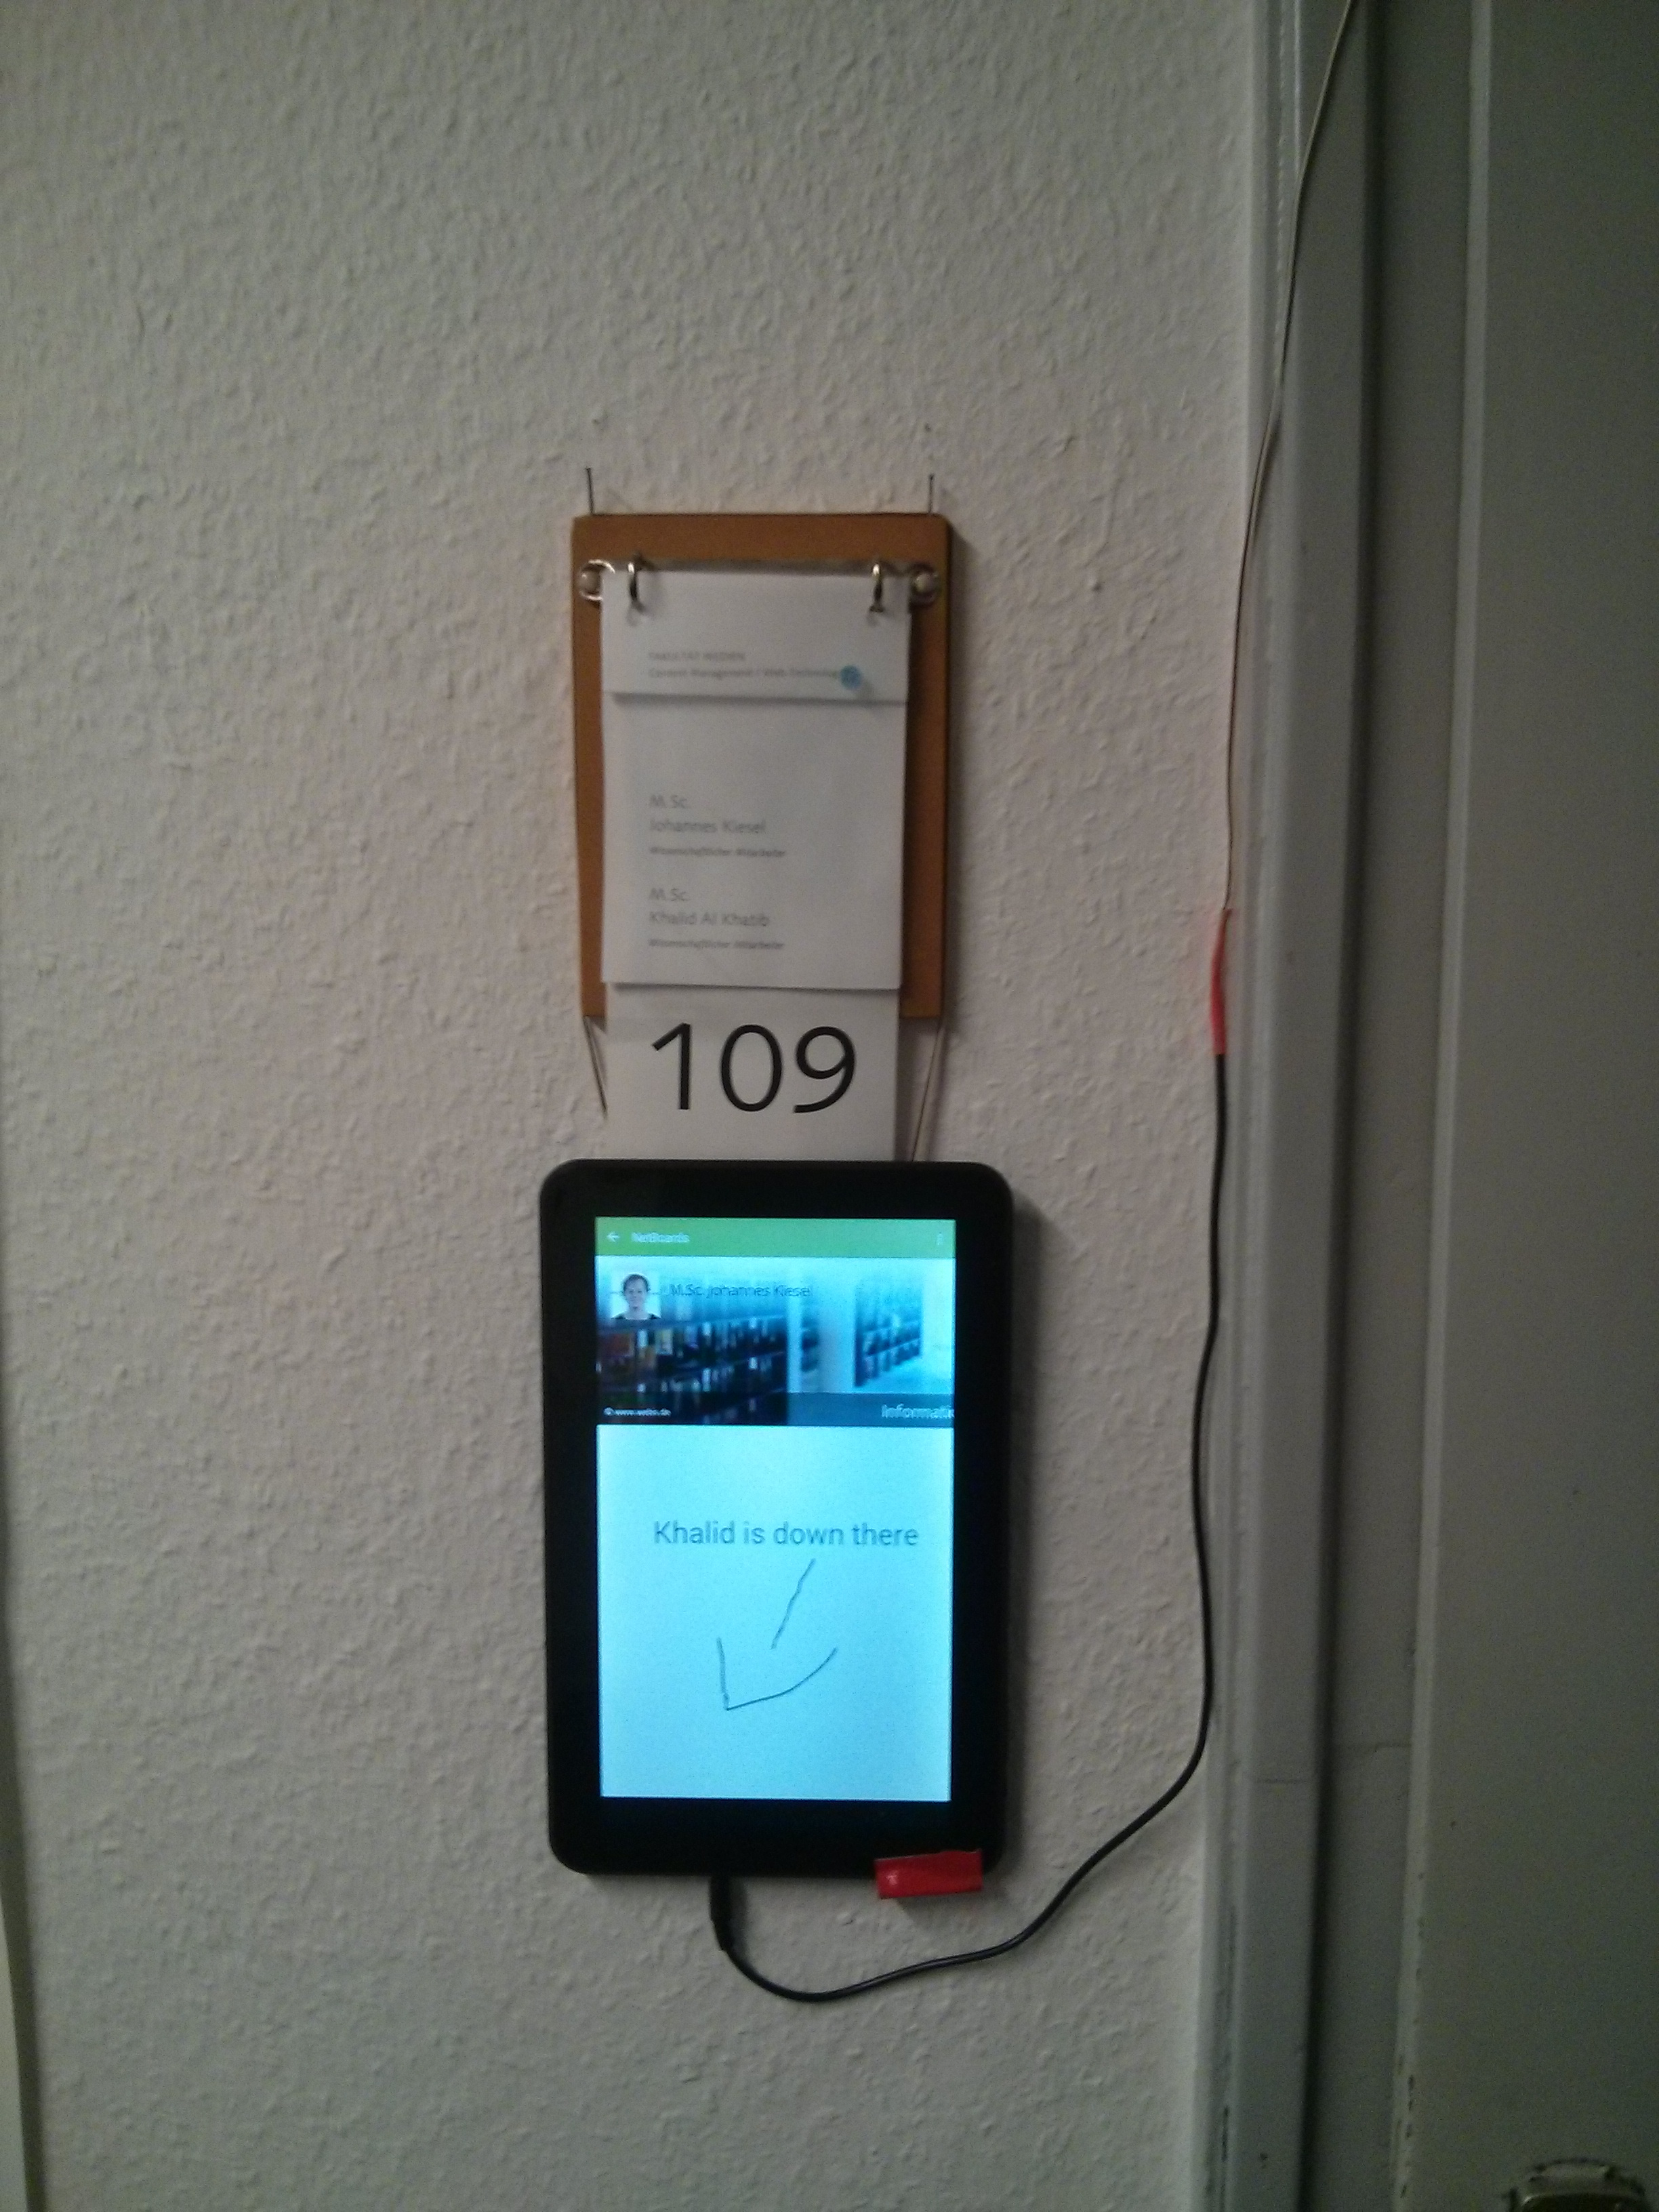
\includegraphics[width=0.9\textwidth]{vorstudie}
    \end{column}
  \end{columns}
  \note<1>{
    \begin{itemize}
      \item Ziel Vorstudie: Anforderungsanalyse des Rahmens der Arbeit
      \item Möglichkeit: Projekt fortsetzen / eigenes Projekt entwickeln
      \begin{itemize}
        \item NetBoards aufgesetzt
        \item Tablet vor Büro in B11 aufgehangen
        \item 1 Woche dauer
      \end{itemize}
    \end{itemize}
  }
  \note<2-3>{
    \begin{itemize}
      \item Ergebnis: Tablet im Gang erzeugte viel Aufmerksamkeit
      \item Durch offene Interaktivität: jeder Gast konnte Inhalt ändern
      \item $\rightarrow$ häufiger Vandalismus (unerwünschter Inhalt)
      \item $\rightarrow$ Projekt nicht fortsetzen 
      \item-click- 
      \item $\rightarrow$ eigenes Projekt erstellen
    \end{itemize}
  }
\end{frame}

  % - Türschilder
  %   - Darbietung von persönlichen Daten (Informationen aller Art - Handskizzen, Texte, Ausdrucke, Statusmeldungen(bin gleich wieder da))
  %   - Kommunikation zwischen Mitarbeitern / Gästen
  % - Problem?:
  %   - Content kann nur geändert werden, wenn man persönlich vor Ort ist
  %   - Zudem können Gäste den bestimmte Sachen abwischen / neue hinzufügen (Vandalismus)
  %   - Hinterlassene Nachrichten können nur gelesen werden, wenn man selbst vor Ort ist
  % - Lösung:
  %   - Interaktive Türschilder
  %   - Digitaler Ersatz für Whiteboards/Tafeln neben Büros
  %   - Nutzer müssen nicht mehr persönlich vor Ort sein, um Content zu ändern / Nachrichten zu empfangen
  %   - Vandalismus wird eingeschränkt

  % - Andere Projekte mit selbem Ansatz
  %   - Hermes (2003)
  %   - Netboards (2014)

  % - Ergebnis aus Vorstudie mit NetBoards: eigenes Projekt

  % wie lange dauert der Abschnitt?? max 10min!!
% \end{frame}
% ---------------------------------------------------------------------
\section{Umsetzung}
% - Bauhausboards
%   * Webapplikation mit Webserver
%   * NodeJS Serverseitig
%   * HTML+CSS+Javascript Clientseitig
%   * Wichtigste Komponente: Editor mit Paper.js
%   * User Frontend + User Backend
%   * wichtigste Funktionen:
%     # User-Content
%     # Messageing System
%     # (beides auf Editor-Grundlage)
%     # Remote-Änderung des Contents
%     # Remote-Einsicht von Messages da per Mail
\begin{frame}{Bauhausboards}
  \begin{center}
    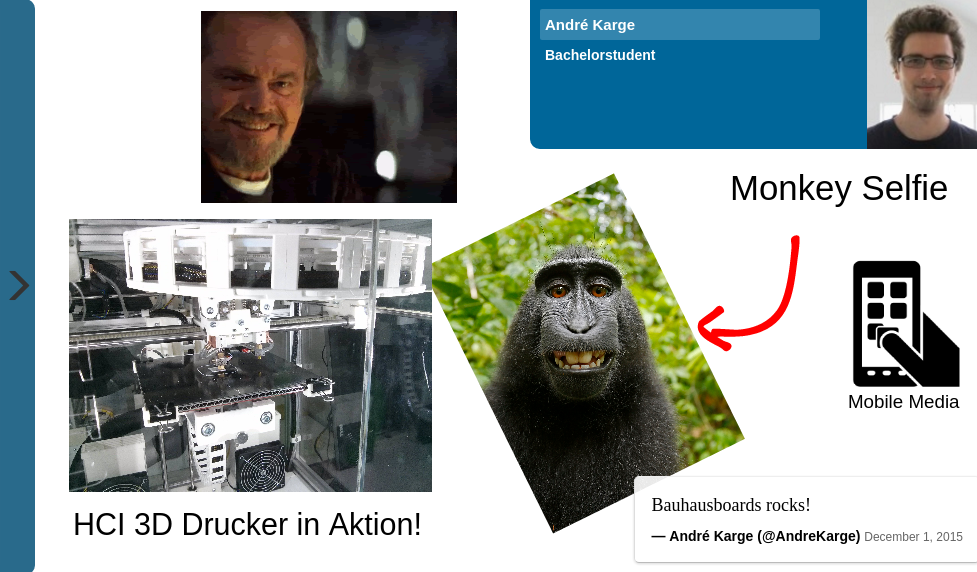
\includegraphics[width=0.9\textwidth]{babo}
  \end{center}
  \note<1>{
    \begin{itemize}
      \item hatte Möglichkeiten: erstellen App für Tablets oder Web-App
      \item Problem Tablet-App: Erhöhter Aufwand durch Portierung zu einzelnen Betriebssystemen
      \item Wohingegen: Jedes Mobile Gerät + PC's Webbrowser haben
      \item Deswegen: Entscheidung: Entwurf von Web-Applikation
      \item System besteht aus: -click-
    \end{itemize}
  }
\end{frame}
\begin{frame}[noframenumbering]{Bauhausboards}
  \begin{center}
    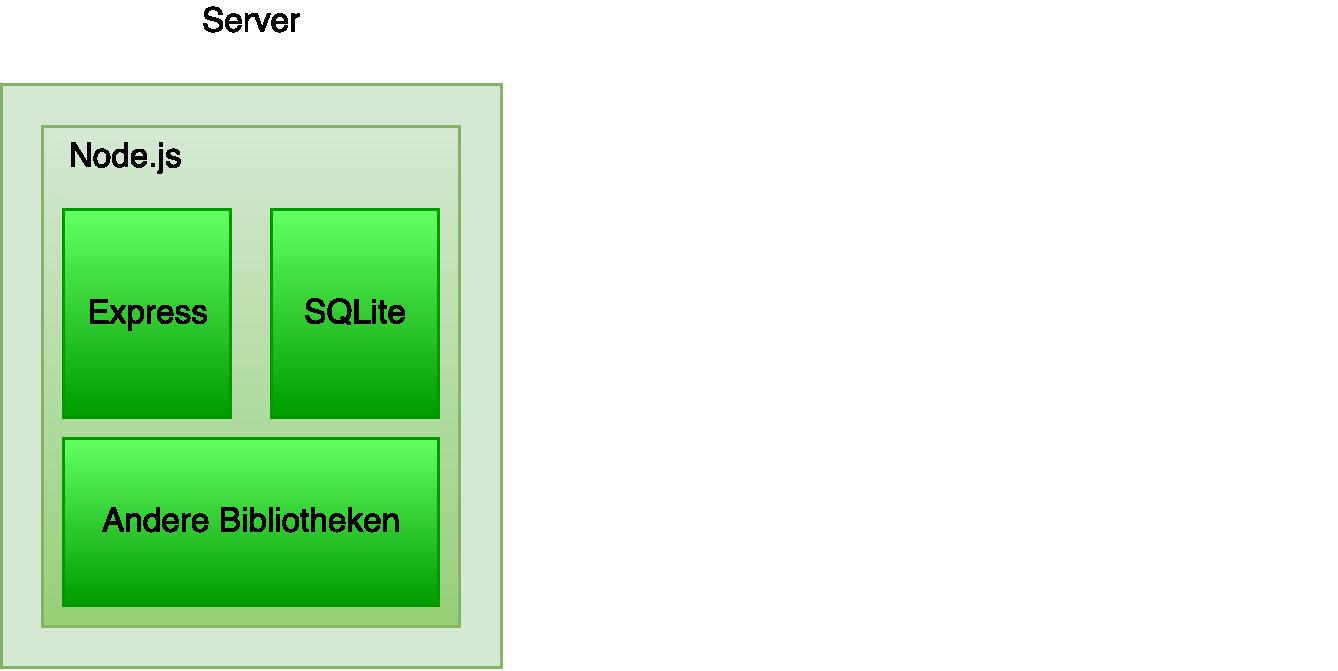
\includegraphics[width=0.9\textwidth]{presBaBo-1.pdf}
  \end{center}
  \note<1>{
    \begin{itemize}
      \item einfacher Webserver (NodeJS Serversprache)
      \item besteht aus mehreren Bibliotheken
      \begin{itemize}
        \item Express = Framework zum Erstellen des Grundgerüsts einer Webseite
        \item SQLite = Datenbank-Bibliothek
        \item mehreren anderen Bibliotheken (Email.js, Crypto.js, twitter.js)
        \item $\rightarrow$ stellen diverse Funktionen bereit
      \end{itemize}
    \end{itemize}
  }
\end{frame}
\begin{frame}[noframenumbering]{Bauhausboards}
  \begin{center}
    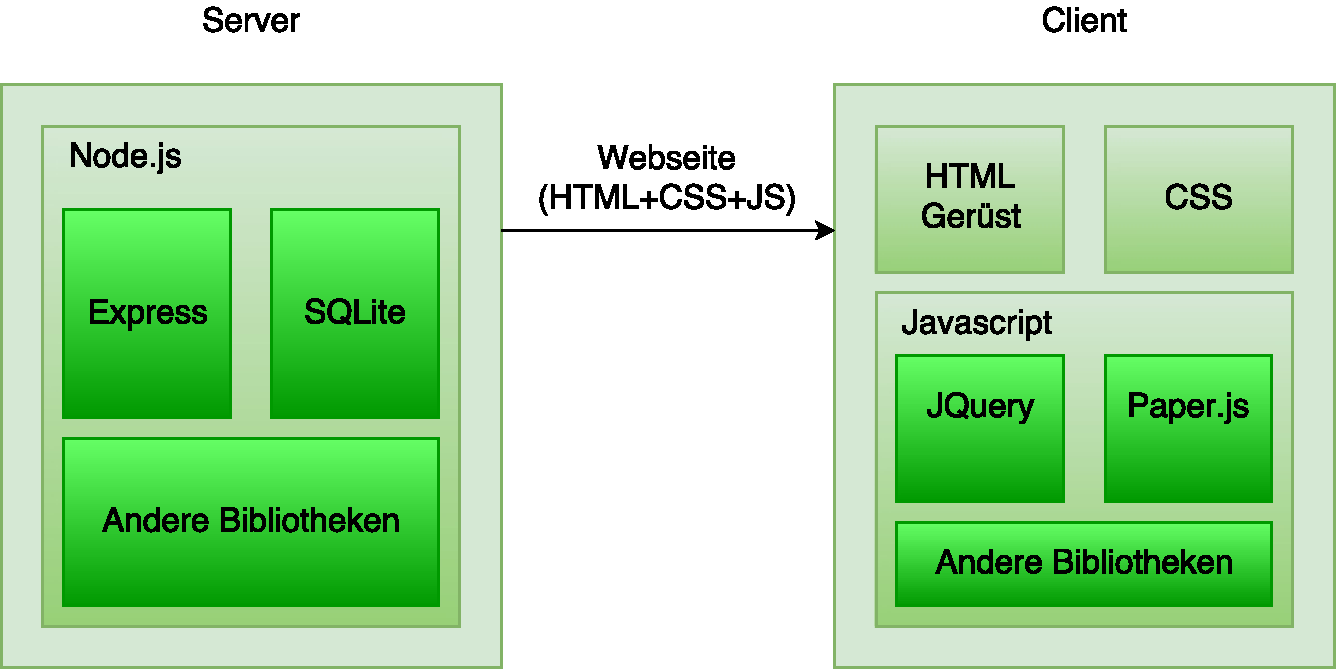
\includegraphics[width=0.9\textwidth]{presBaBo-2.pdf}
  \end{center}
  \note<1>{
    \begin{itemize}
      \item Webserver liefert Webseite an Clients aus
      \item Webseite besteht aus dem Express-Grundgerüst + CSS + allen Javascript Funktionen
      \item Javascript-Funktionalität hauptsächlich:
      \begin{itemize}
        \item JQuery zur Manipulation des Seitenaufbaus+Datenaustausch mit Server
        \item Paper.js (Editor basiert darauf)
        \item andere kleinere Bibliotheken
        \item -click-
      \end{itemize}
    \end{itemize}
  }
\end{frame}
\begin{frame}[noframenumbering]{Bauhausboards}
  \begin{center}
    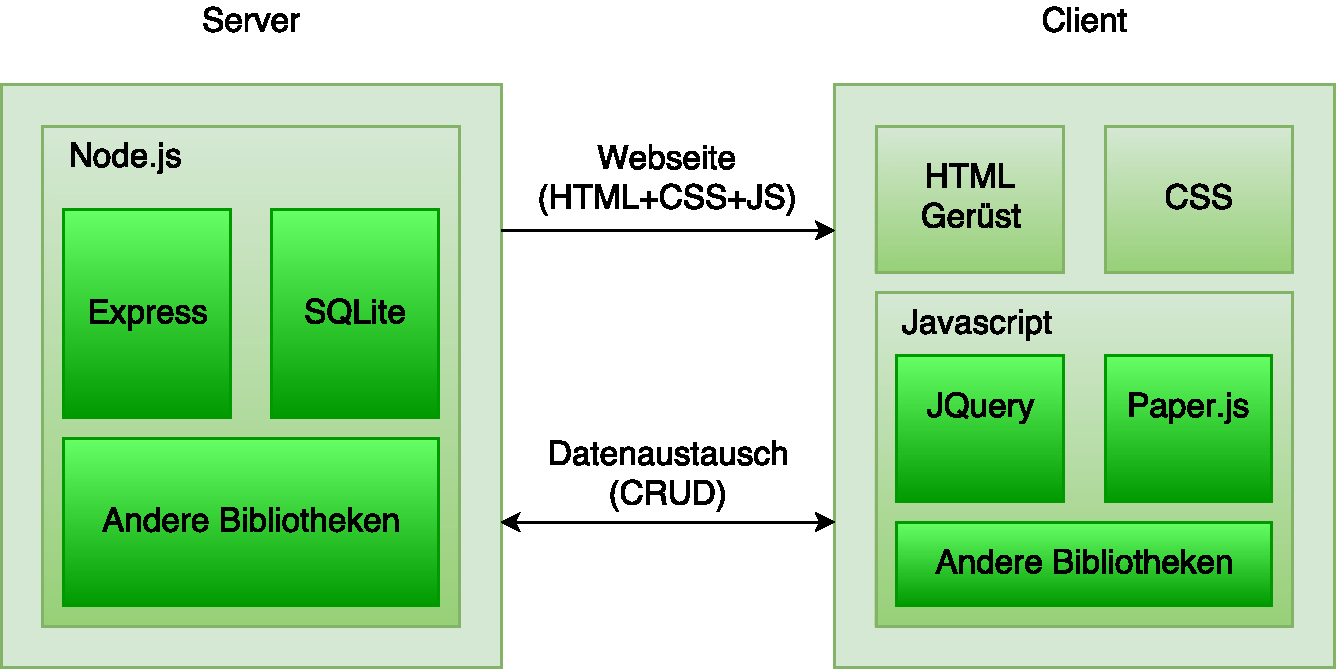
\includegraphics[width=0.9\textwidth]{presBaBo-3.pdf}
  \end{center}
  \note<1>{
    \begin{itemize}
      \item Datenaustausch mit Server per Ajax über CRUD-Prinzip\\(C(create) R(ead) U(pdate) D(elete))
      \item daten werden dynamisch nachgeladen + Seite muss nicht neu geladen werden
    \end{itemize}
  }
\end{frame}

\begin{frame}[t]{Hauptfunktionen}
  \begin{columns}
    \begin{column}[t]{0.49\textwidth}
      \begin{center}
        \visible<1-4>{
          \textbf{Nutzerinhalt}
        }
        \visible<3-4> {
          \begin{itemize}
            \item Jeder Nutzer hat eigene Pinnwand
            \item Informationen für alle Gäste sichtbar
            \item Nur Nutzer können Inhalt ändern
          \end{itemize}
        }
      \end{center}
    \end{column}
    \begin{column}[t]{0.49\textwidth}
      \begin{center}
        \visible<2-4>{
          \textbf{Nachrichtensystem}
        }
        \visible<4>{
          \begin{itemize}
            \item Jeder Gast kann Nachricht schreiben
            \item Mitarbeiter bekommt Nachricht als Email
            \item Nur Autor und Empfänger kennen Nachrichteninhalt
          \end{itemize}
        }
      \end{center}
    \end{column}
  \end{columns}
  \note<1-2>{
    \begin{itemize}
      \item Hauptfunktionen von Bauhausboards sind:
      \item Erstellung Nutzerinhalt durch Mitarbeiter im Büro
      \item -click-
      \item Kommunikationsmöglichkeit über Nachrichtensystem von Gästen an Mitarbeiter
      \item -click-
    \end{itemize}
  }
  \note<3>{
    Nutzerinhalt:
    \begin{itemize}
      \item jeder Mitarbeiter hat eigene Pinnwand im System
      \item $\rightarrow$ darbietung von eigenem Erstelltem Inhalt (Text, Skizzen, Bilder, Gifs, Webseiten)
      \item Informationen für alle Gäste sichtbar
      \item Nutzer muss sich anmelden, um Inhalt zu ändern
      \item kein anderer kann Inhalt ändern
    \end{itemize}
  }
  \note<4>{
    Nachrichtensystem:
    \begin{itemize}
      \item jeder vorbeilaufende Gast/Mitarbeiter kann bestimmten Mitarbeitern im Raum Nachricht hinterlassen
      \item bspw.: wenn Mitarbeiter grad nicht da ist / Konferenz hat
      \item Wenn nachricht abgeschickt: Mitarbeiter bekommt Email
      \item Vorteil: Gast kann Mitarbeiter schnell vor Ort Email schreiben
      \item Vorteil: nur autor + empfänger kennen Nachrichteninhalt
    \end{itemize}
  }
\end{frame}

\begin{frame}{Editor}

  Anforderungen:\\
  \pause
  \begin{columns}[t]

    \begin{column}{0.24\textwidth}
      \begin{center}
        \textbf{Zeichnen}\\mit\\verschieden-\\farbigen Stiften
      \end{center}
    \end{column}
    \pause
    \begin{column}{0.24\textwidth}
      \begin{center}
        \textbf{Anheften}\\von\\Bildern und Zetteln
      \end{center}
    \end{column}
    \pause
    \begin{column}{0.24\textwidth}
      \begin{center}
        \textbf{Neuanordnen}\\von\\Bildern und Zetteln
      \end{center}
    \end{column}
    \pause
    \begin{column}{0.24\textwidth}
      \begin{center}
        \textbf{Entfernen}\\von\\Zeichnungen, Bildern und Zetteln
      \end{center}
    \end{column}
  \end{columns}


  \note<1-5>{
    \begin{itemize}
      \item Hauptkomponente von Bauhausboards = Editor
      \item sollte annähernd Funktionen von Tafel/Whiteboard haben -click-
      \begin{itemize}
        \item Zeichnen mit verschiedenfarbigen Stiften (unterschiedlicher Dicke)
        \item Anheften von Bildern/Zetteln (per Magnet oder Pinnadel)
        \item Neuanordnung angehefteter Elemente
        \item Entfernen von gezeichneten Elementen (Schwammfunktion / Zettel entfernen)
      \end{itemize}
    \end{itemize}
  }
\end{frame}
\begin{frame}{Editor}
  \begin{center}
    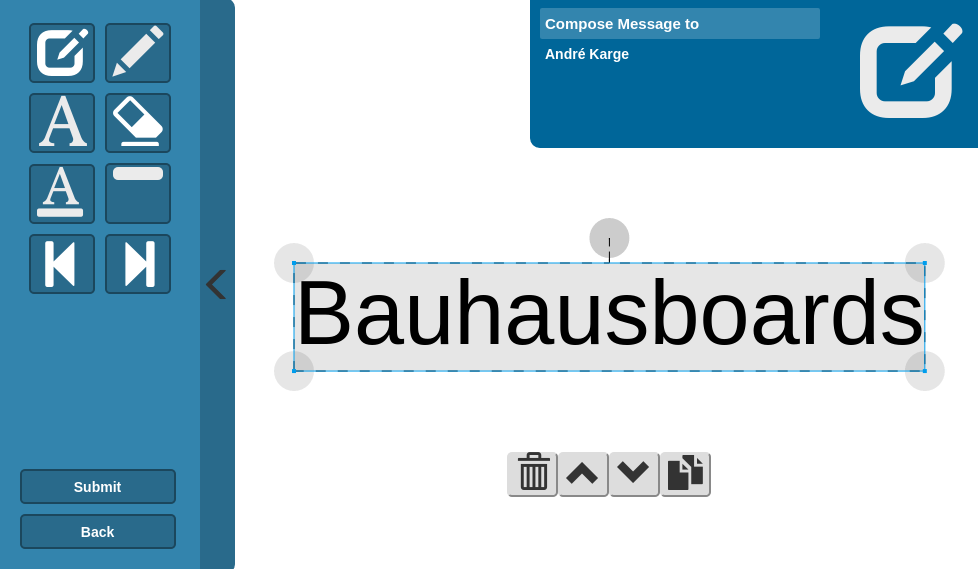
\includegraphics[width=0.9\textwidth]{editor}
  \end{center}
  \note<1>{
    \begin{itemize}
      \item realisiert Javascript-Framework: Paper.js
      \item da paper.js nur Framework zur Darstellung von Vektorgrafiken:
      \item passender Editor selbst implementiert
      \item Alle Anforderungen an Whiteboard/Tafel erfüllt
      \item + Zusatzfunktionen (UNDO+REDO, nachträgliches Ändern von Farbe, Neuanordnung von Zeichnungen)
    \end{itemize}
  }
\end{frame}
\begin{frame}{Vorteile Bauhausboards}
  \begin{itemize}
    \item Von Überall erreichbar
    \pause
    \item Erhöhte Sicherheit vor Vandalismus
    \pause
    \item Darstellung von animiertem Inhalt
  \end{itemize}
  \note<1-3>{
    \begin{itemize}
      \item Da man von Überall auf den Server zugreifen kann: nicht notwendig direkt vor Ort zu sein
      \item -click-
      \item Sicherheitsaspekt, da nur angemeldete Nutzer präsentierten Inhalt ändern können
      \item -click-
      \item Präsentation von Animierten Inhalten (zur Zeit nur Gifs)
    \end{itemize}
    (System musste auf Nutzbarkeit getestet werden)
  }
\end{frame}

  % - Bauhausboards
  % - Web-Applikation
  %   - Serverseitig
  %     - NodeJS für Serversprache
  %     - SQLite für Datenbank
  %   - Clientseite
  %     - HTML+CSS Webseite ausgeliefert
  %     - Javascript mit JQuery für HTML-DOM Manipulation und Funktionalitäten
  %   - Kommunikation Client-Server
  %     - erster Aufruf liefert Webseite und Funktionalitäten (JS) aus
  %     - Dynamisches Nachladen von Daten per Ajax (CRUD Prinzip)
  %   - Komponenten
  %     - Editor - Da Simulation von Tafel/Whiteboard
  %       - Editorfunktionen
  %         - Zeichnen mit verschiedenfarbigen Stiften
  %         - Schwammfunktion zum Entfernen von gezeichneten/geschriebenen Elementen
  %         - Anheften von Bildern/Zetteln per bspw.: Magneten
  %         - Neuanordnung von angehefteten Elementen
  %       - realisiert mit dem Javascript-Framework Paper.js
  %     - Nutzerinhalt(auf Basis von Editor)
  %     - Nachrichtensystem(auf Basis von Editor)
  %   - Vorteile gegenüber Whiteboards/Tafeln:
  %     - Da man von Überall auf den Server zugreifen kann: nicht notwendig direkt vor Ort zu sein
  %     - Sicherheitsaspekt, da nur angemeldete Nutzer präsentierten Inhalt ändern können
  %     - Präsentation von Animierten Inhalten (zur Zeit nur Gifs)
  % - Überleitung zur Studie
  %   - Das System musste auf Nutzbarkeit getestet werden
% \end{frame}
% ---------------------------------------------------------------------
\section{Studie}
% - Studie
%   * System musste getestet werden
%   * 9 Tester á 4 Räume via 4 Tablets
%   * Tutorial mit allen Funktionen erstellt
%   * 2 Wochen Laufzeit
%   * Auswertung der Studie
%     # Interview zum Sammeln von Feedback (Anzahl von Fragen mit angeben vllt noch Beispielfragen)
%     # UEQ Fragebogen
\begin{frame}{Testsystem}
  \begin{columns}
    \begin{column}{0.49\textwidth}
      \begin{itemize}
        \item 1 Webserver
        \item 4 Tablets
        \item 9 Probanden
        \item 2 Wochen Laufzeit
      \end{itemize}
    \end{column}
    \begin{column}{0.49\textwidth}
      \begin{center}
        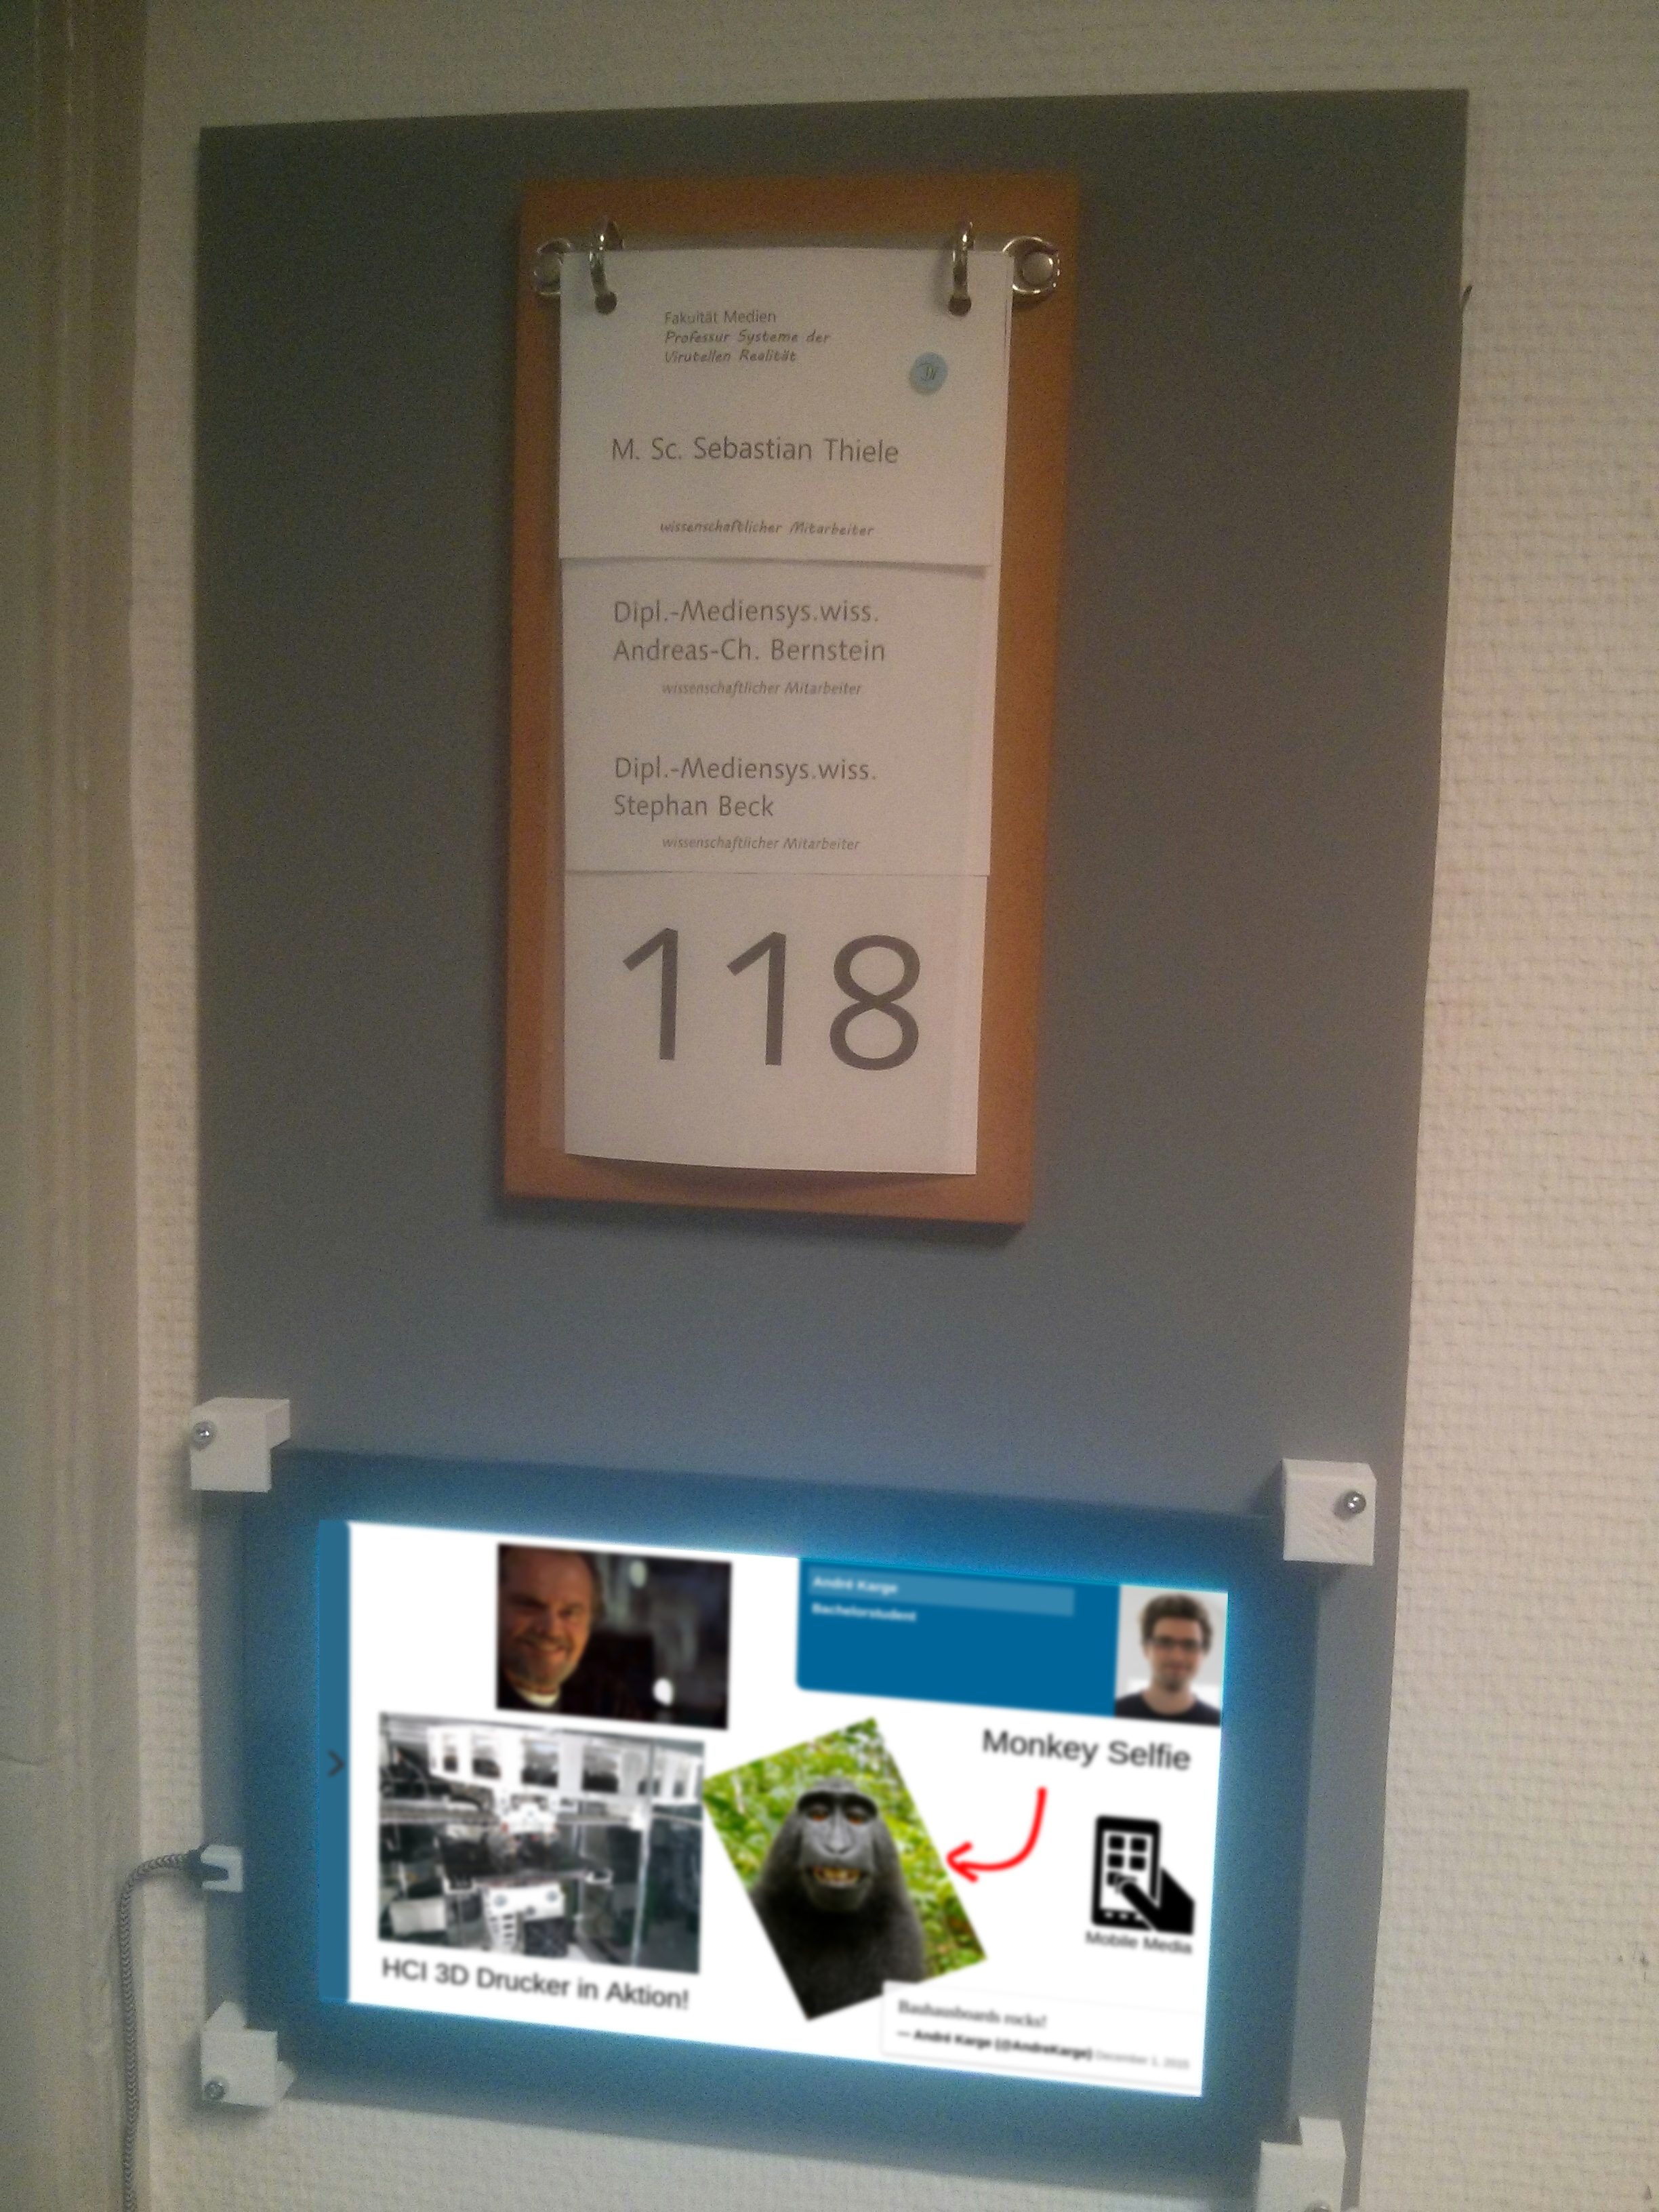
\includegraphics[width=0.9\textwidth]{schild2}
      \end{center}
    \end{column}
  \end{columns}
  \note<1>{
    \begin{itemize}
      \item Dazu: Testsystem aufgesetzt
      \item 1 Webserver + 4 Tablets mit Webrowser im Kiosk-Mode
      \item Tablets vor 4 Räumen in der Bauhausstraße 11 angebracht (9 Probanden)
      \item Laufzeit: 2 Wochen
      \item Zudem: Tutorial-Dokument mit Erklärung zu allen Funktionen aufgesetzt
    \end{itemize}
  % - Testsystem aufgesetzt\\
  %   - Webserver\\
  %   - 4 Tablets mit Webprowser im Kiosk-Modus\\
  % - How-To-Pdf aufgestzt, mit allen Funktionen des System und wie sie zu benutzen sind\\
  % - Tablets vor Büros in der Bauhausstraße 11 angebracht\\
  % - Studienlaufzeit: 2 Wochen\\
  }
\end{frame}

\begin{frame}{Auswertung}
  % \begin{columns}
  %   \begin{column}{0.49\textwidth}
  %     \begin{center}
  %       {\large Interview}
  %     \end{center}
  %   \end{column}
  %   \begin{column}{0.49\textwidth}
  %     \begin{center}
  %       {\large UEQ}
  %     \end{center}
  %   \end{column}
  % \end{columns}
  Interview
  \begin{itemize}
    \item Probanden mit Fragenkatalog befragt
    \item 5h 30min an Audiomitschnitten
  \end{itemize}
  \pause
  UEQ (User-Experience-Questionaire)
  \begin{itemize}
    \item Zusätzliche Auswertung
    % \item 
  \end{itemize}
  \note<1>{
    \begin{itemize}
      \item Um Studie auszuwerten:
      \item Entwurf Interview
      \item $\rightarrow$ Fragenkatalog - Fragen zu bestimmten Systemfunktionen
      \item Probanden wurden nach Studie befragt
      \item interviews mitegeschnitten $\rightarrow$
      \item 5h 30min Interview Mitschnitte (spätere Analyse)
    \end{itemize}
  }
  \note<2>{
      \begin{itemize}
      \item Zusätzlich: UEQ(User-Experience-Questionaire) Fragebogen ausfüllen als zusätzliche Auswertung
      \item Da nur 9 Probanden: Aussagekraft von UEQ recht schwach
      \item Mehr Feedback durch Interviews erhalten
    \end{itemize}
  }
\end{frame}

\begin{frame}{Studienergebnisse}
  \begin{columns}
    \begin{column}[t]{0.49\textwidth}
      Nutzer erzeugten diverse Inhalte:\\
      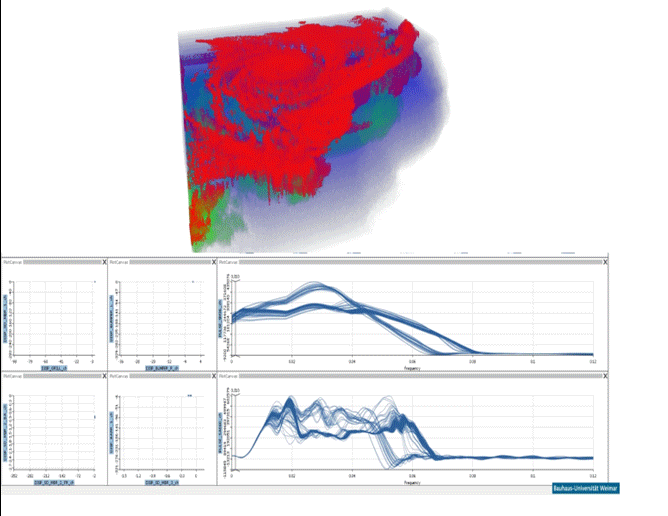
\includegraphics[width=0.9\textwidth]{content_ex}\\
      \quelle{Quelle: Sebastian Thiele}
    \end{column}
    \visible<2> {
      \begin{column}[t]{0.49\textwidth}
        Gäste hinterließen Nachrichten:\\
        
\includegraphics[width=0.9\textwidth]{message_ex}
      \end{column}
    }
  \end{columns}
  \note<1-2>{
    \begin{itemize}
      \item Nutzer: diverse Inhalte (größtenteils Spaß-Inhalte / auch: Information zu aktueller Arbeit)
      \item Beispiel aus Studie: ein animiertes Gif zur darstellung einer Vektorfeldvisualisierung
      \item -click-
      \item Gäste: hinterließen Nutzern viele Nachrichten (zum Teil mit Kontext / aber: zum teil ohne)
      \item Beispiel aus Studie: Ein Gast/Mitarbeiter fragt Nutzer zum Essen gehen
    \end{itemize}
  }
\end{frame}

\begin{frame}{Studienergebnisse}
  Pro:
  \visible<2-3>{
    \begin{itemize}
      \item Darstellung von animiertem Inhalt
      \item Nachrichten mit persönlicher Note
      \item Anpassung des Inhaltes aus der Ferne
    \end{itemize}
  }
  Contra:
  \visible<3>{
    \begin{itemize}
      \item Studie zu kurz
      \item Keine Autorenkennzeichnung in Mitteilungen
      \item Eingebaute Authentisierungsmethoden hinderlich
    \end{itemize}
  }
  \note<1>{
    \begin{itemize}
      \item als Ergebnis der Interviews: gewisse Vor- / Nachteile
    \end{itemize}
  }
  \note<2>{
    Nutzer empfanden:
    \begin{itemize}
      \item bestes Feature: Darstellung von Gifs
      \item Emails durch Skizzen: persönliche Note
      \item Außerdem: gut aufgenommen: Inhaltsänderung per Remote ohne selbst vor Ort / Beauftragung Kollegen
    \end{itemize}
  }
  \note<3>{
    Nutzer bemängelten:
    \begin{itemize}
      \item Leider: Studie ein wenig zu kurz $\rightarrow$ Nutzer konnten sich nicht vollständig an System gewöhnen
      \item größtes Manko: fehlen von Authorenkennzeichnung in Nachrichten
      \item zudem: hatte 2 Authentisierungsmethoden eingebaut\\
            $\rightarrow$ tester fanden interaktion hinderlich
    \end{itemize}
  }
\end{frame}
%   - Testsystem aufgesetzt
%     - Webserver
%     - 4 Tablets mit Webprowser im Kiosk-Modus
%   - How-To-Pdf aufgestzt, mit allen Funktionen des System und wie sie zu benutzen sind
%   - Tablets vor Büros in der Bauhausstraße 11 angebracht
%   - Studienlaufzeit: 2 Wochen
%     - dabei:
%       - Nutzer erzeugten diverse Inhalte(meistens Fun aber auch informativ)
%       - Gäste hinterließen Nutzern Nachrichten (dabei aber auch ab und an ohne Kontext/ temporäres Graffiti)
%   - Auswertung der Studie durch Interviews + Fragebogen
%     - 5h 30min an Interview-Mitschnitten zur besseren Analyse
%     - Fragenkatalog mit Fragen zu bestimmten Systemfunktionen
%     - UEQ (User-Experience-Questionaire) als Standardevaluationsmethode
%   - Ergebnisse der Studie
%     - wurde größtenteils wegen der Möglichkeit bewegten Inhalt zu erstellen genutzt (das heißt viele Gifs usw.)
%     - 2 Eingebaute Authentisierungsmethoden waren hinderlich
%     - einigen Nutzern waren manche Schritte zu kompliziert
%     - Authorenkennzeichnung in Nachrichten hat gefehlt (größtes Manko)
%     - Emails bekommen durch Skizzen eine persönliche Note
% \end{frame}
% ---------------------------------------------------------------------
\section{Ausblick}
% - Ausblick
%   * Strukturänderungen am System (Frontend - Backend Trennung) - als Konsequenz der Studie
%   * Poweruser Einstellung
%   * Audio-/Video-/Fotonachrichten
\begin{frame}{Ausblick}
  Änderungen am System\pause:
  \begin{itemize}
    \item Neue Nachrichtentypen
    \item Strukturänderungen
    \item Poweruser-Funktion
  \end{itemize}
  \pause
  \bigskip
  Durchführung einer weiteren, größeren Studie
  \note<1-3>{
    \begin{itemize}
      \item aus Studienergebnissen: Schlussfolgerungen:
      \item Änderungen am System
      \item Einbau neuer Nachrichtentypen: Audio-/Video-/Fotonachrichten (Autorenproblem)
      \item Strukturänderungen am System: Tablets nur noch als Kommunikationskanal nutzen $\rightarrow$ Trennung Frontend-Backend (Authentisierungsproblem)
      \item Hinzufügung einer Poweruser-Funktion (Kapselung komplexerer Funktionen) $\rightarrow$ Standardnutzer sollen nicht von Zusatzfunktionen erdrückt werden
      \item Durchführung einer weiteren Studie (länger + mehr Probanden) 
    \end{itemize}
  }
\end{frame}
% ---------------------------------------------------------------------

\section{Demo}

\AtBeginSection{}
\section*{Ende}

\subsection*{}
\begin{frame}
  \begin{centering}
    \begin{beamercolorbox}[sep=12pt,center]{part title}
      \usebeamerfont{section title}{Fragen?}\par
    \end{beamercolorbox}
  \end{centering}
\end{frame}
\subsection*{}
\begin{frame}
  \begin{centering}
    \begin{beamercolorbox}[sep=12pt,center]{part title}
      \usebeamerfont{section title}{Danke für Ihre Aufmerksamkeit!}\par
    \end{beamercolorbox}
  \end{centering}
\end{frame}

\end{document}
